В \underline{\textbf{четвёртой главе}} проведён анализ и учёт внешних факторов, влияющих на точность определения коэффициента оптического поглощения нелинейно-оптических кристаллов методом лазерной калориметрии, в частности, пьезоэлектрической резонансной лазерной калориметрии (ПРЛК). Предложены поправочные выражения для экспоненциальной, импульсной и градиентной методик обработки температурных кинетик, компенсирующие неконтролируемые изменения температуры окружающей среды и коэффициента теплоотдачи. Экспериментально подтверждено, что применение разработанных поправок снижает максимальный разброс значений коэффициента поглощения, полученных различными методиками, с 23\% до 11\%.

Стандартное уравнение теплового баланса предполагает постоянство температуры окружающей среды $T_a$ и коэффициента теплоотдачи $\Gamma$. В общем случае эти параметры зависят от времени, и уравнение принимает вид:

\begin{equation}
	\begin{cases}
		\dfrac{d T}{d t} = \overline{Q}\theta(t_0 - t) - \Gamma(t)(T - T_a(t)), \\
		T(0) = T_a(0),
	\end{cases}
	\label{eq:syno_balance_equation_timed}
\end{equation}

Для оценки влияния временных зависимостей $T_a(t)$ и $\Gamma(t)$ на погрешность определения коэффициента поглощения задавались их конкретные виды, уравнение решалось численно, после чего определялось отклонение восстановленного коэффициента от заданного. В качестве модельного образца выбран кристалл LBO с размерами $1\times1\times5$~см$^3$ и радиусом пучка 1 мм на длине волны 1030~нм. Выбор кристалла обусловлен его широким применением для нелинейного преобразования высоких средних мощностей, а геометрия образца обеспечивает усиление влияния тепловых эффектов для корректной верификации поправок.

Изменение температуры окружающей среды во времени вносит дополнительный член в уравнение теплового баланса:
\begin{equation}
	\overline{Q}\theta(t - t_0) \rightarrow \overline{Q}\theta(t - t_0) - d T_a/d t.
	\label{eq:syno_q_corr_ta}
\end{equation}

Для градиентного метода учёт температурных флуктуаций сводится к поправке:
\begin{equation}
	G_{corr} = G - \left(\frac{d T_a}{d t} \bigg|_{t < t_0, T = T_0} - \frac{d T_a}{dt} \bigg|_{t > t_0, T = T_0}\right).
	\label{eq:syno_g_corr_ta}
\end{equation}

Для экспоненциального и импульсного методов коррекция выполняется путём разложения $T_a(t)$ в ряд Фурье. Решение уравнения теплового баланса для гармонической компоненты $\hat{T}_a(\omega) \exp(i\omega t)$ даёт добавку к температурной кинетике:

\begin{equation}
	\epsilon(t) = \sum_{\omega_k} \dfrac{i\omega_k \hat{T}_a(\omega_k)}{\Gamma + i\omega_k} [\exp(-\Gamma t) - \exp(i\omega_k t)].
	\label{eq:syno_correction_ta}
\end{equation}

Эта поправка вычитается из экспериментальной кинетики перед аппроксимацией. Расчёт поправки требует знания $\Gamma$, что обуславливает итерационную процедуру.

\begin{figure}[h!]
	\centering
	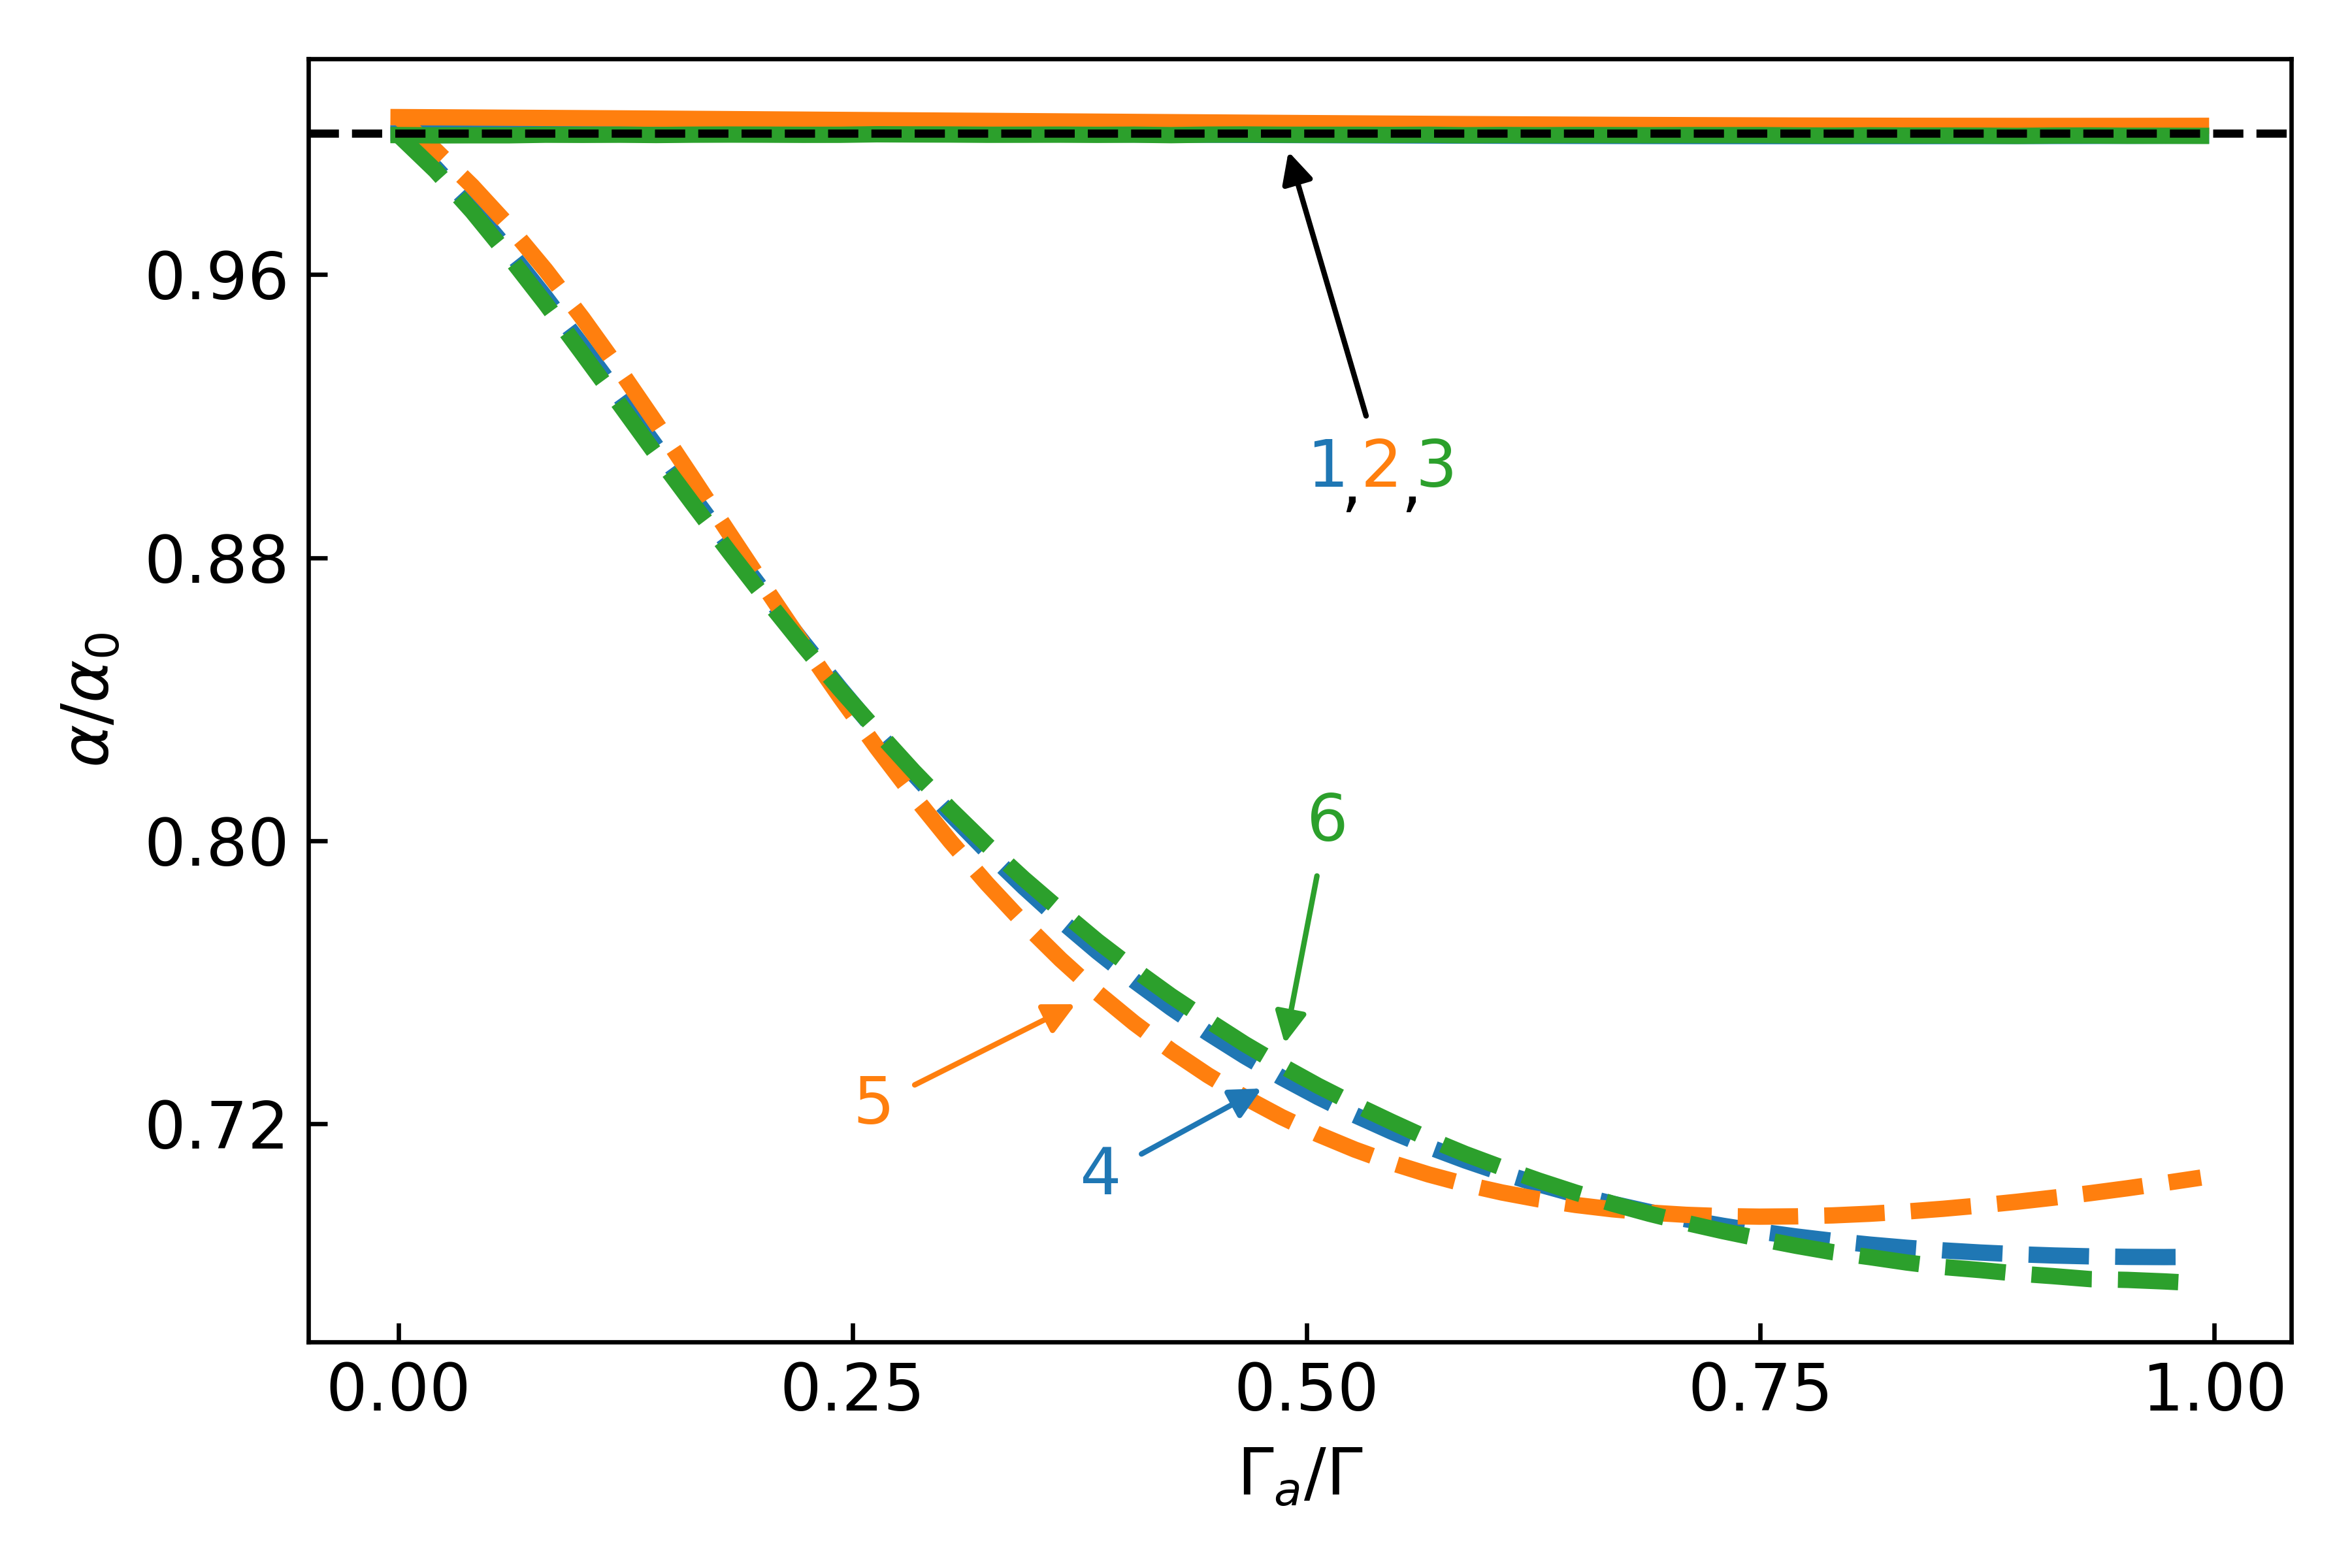
\includegraphics[width=0.85\linewidth]{Dissertation/images/gradient/fourier_ambient_exp}
	\caption{Зависимость погрешности определения коэффициента поглощения от отношения скоростей теплоотдачи окружающей среды и кристалла $\Gamma_a/\Gamma$. Кривые 1--3 — методы с учётом поправки; кривые 4--6 — без коррекции.}
	\label{fig:syno_correction_ta}
\end{figure}

На рис.~\ref{fig:syno_correction_ta} представлена зависимость погрешности от отношения $\Gamma_a/\Gamma$. При $\Gamma_a/\Gamma \rightarrow 1$ погрешность превышает 30\%, а применение поправки снижает её до уровня порядка 1\%.